\documentclass{standalone}

\usepackage[OT1]{fontenc}
\renewcommand*\familydefault{\sfdefault}
\usepackage{helvet,sfmath}
\usepackage{siunitx}

\usepackage{tikz}
\usetikzlibrary{arrows,calc,patterns}
% \usetikzlibrary{intersections, calc, arrows.meta}
\usepackage{tikz,tkz-euclide}

\begin{document}
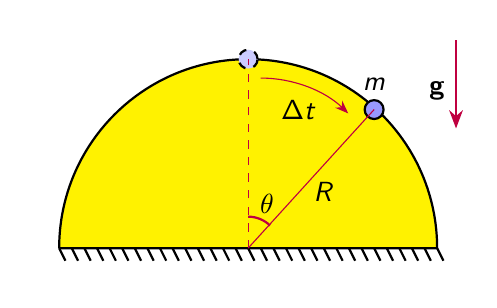
\begin{tikzpicture}[scale=0.8, >=Stealth]

    %% Background
    \draw[draw=none] (-3.5,-0.5) rectangle (3.5,3.5);

    %Hemisphere
    \draw[thick, fill=yellow] (-3,0) arc(180:0:3) to (-3,0);

    \foreach \x in {-3,-2.8,...,2.8,3}
    {
    \draw[thick] (\x,0) to (\x+0.1,-0.2);
    }

    % Point
    \draw[thick, fill=blue!40] (2,2.2) circle (0.15);

    \draw[fill=blue!20, thick, dashed] (0,3) circle (0.15);

    % Coordinate
    \draw[dashed, purple]
    (0,0) to (0,3)
    ;
    \draw[purple]
    (0,0) to (2,2.2)
    ;

    \draw[thick, purple]
    (0,0.5) arc(90:46:0.5)
    ;

    \draw[thick, purple, -Stealth] (3.3,3.3) to (3.3,1.9);

    \draw[purple, -Stealth] (0.2,2.7) arc(90:46:2);
    
    \draw
    (0.3,0.7) node{\(\theta\)}
    (1.2,0.9) node{\(R\)}
    (3,2.5) node{\(\mathbf{g}\)}
    (2.0,2.6) node{\(m\)}
    (0.8,2.2) node{\(\Delta t\)}
    ;
    
\end{tikzpicture}
\end{document}